\documentclass[]{article}
\usepackage{lmodern}
\usepackage{amssymb,amsmath}
\usepackage{ifxetex,ifluatex}
\usepackage{fixltx2e} % provides \textsubscript
\ifnum 0\ifxetex 1\fi\ifluatex 1\fi=0 % if pdftex
  \usepackage[T1]{fontenc}
  \usepackage[utf8]{inputenc}
\else % if luatex or xelatex
  \ifxetex
    \usepackage{mathspec}
    \usepackage{xltxtra,xunicode}
  \else
    \usepackage{fontspec}
  \fi
  \defaultfontfeatures{Mapping=tex-text,Scale=MatchLowercase}
  \newcommand{\euro}{€}
\fi
% use upquote if available, for straight quotes in verbatim environments
\IfFileExists{upquote.sty}{\usepackage{upquote}}{}
% use microtype if available
\IfFileExists{microtype.sty}{%
\usepackage{microtype}
\UseMicrotypeSet[protrusion]{basicmath} % disable protrusion for tt fonts
}{}
\ifxetex
  \usepackage[setpagesize=false, % page size defined by xetex
              unicode=false, % unicode breaks when used with xetex
              xetex]{hyperref}
\else
  \usepackage[unicode=true]{hyperref}
\fi
\hypersetup{breaklinks=true,
            bookmarks=true,
            pdfauthor={},
            pdftitle={},
            colorlinks=true,
            citecolor=blue,
            urlcolor=blue,
            linkcolor=magenta,
            pdfborder={0 0 0}}
\urlstyle{same}  % don't use monospace font for urls
\usepackage{color}
\usepackage{fancyvrb}
\newcommand{\VerbBar}{|}
\newcommand{\VERB}{\Verb[commandchars=\\\{\}]}
\DefineVerbatimEnvironment{Highlighting}{Verbatim}{commandchars=\\\{\}}
% Add ',fontsize=\small' for more characters per line
\newenvironment{Shaded}{}{}
\newcommand{\KeywordTok}[1]{\textcolor[rgb]{0.00,0.44,0.13}{\textbf{{#1}}}}
\newcommand{\DataTypeTok}[1]{\textcolor[rgb]{0.56,0.13,0.00}{{#1}}}
\newcommand{\DecValTok}[1]{\textcolor[rgb]{0.25,0.63,0.44}{{#1}}}
\newcommand{\BaseNTok}[1]{\textcolor[rgb]{0.25,0.63,0.44}{{#1}}}
\newcommand{\FloatTok}[1]{\textcolor[rgb]{0.25,0.63,0.44}{{#1}}}
\newcommand{\ConstantTok}[1]{\textcolor[rgb]{0.53,0.00,0.00}{{#1}}}
\newcommand{\CharTok}[1]{\textcolor[rgb]{0.25,0.44,0.63}{{#1}}}
\newcommand{\SpecialCharTok}[1]{\textcolor[rgb]{0.25,0.44,0.63}{{#1}}}
\newcommand{\StringTok}[1]{\textcolor[rgb]{0.25,0.44,0.63}{{#1}}}
\newcommand{\VerbatimStringTok}[1]{\textcolor[rgb]{0.25,0.44,0.63}{{#1}}}
\newcommand{\SpecialStringTok}[1]{\textcolor[rgb]{0.73,0.40,0.53}{{#1}}}
\newcommand{\ImportTok}[1]{{#1}}
\newcommand{\CommentTok}[1]{\textcolor[rgb]{0.38,0.63,0.69}{\textit{{#1}}}}
\newcommand{\DocumentationTok}[1]{\textcolor[rgb]{0.73,0.13,0.13}{\textit{{#1}}}}
\newcommand{\AnnotationTok}[1]{\textcolor[rgb]{0.38,0.63,0.69}{\textbf{\textit{{#1}}}}}
\newcommand{\CommentVarTok}[1]{\textcolor[rgb]{0.38,0.63,0.69}{\textbf{\textit{{#1}}}}}
\newcommand{\OtherTok}[1]{\textcolor[rgb]{0.00,0.44,0.13}{{#1}}}
\newcommand{\FunctionTok}[1]{\textcolor[rgb]{0.02,0.16,0.49}{{#1}}}
\newcommand{\VariableTok}[1]{\textcolor[rgb]{0.10,0.09,0.49}{{#1}}}
\newcommand{\ControlFlowTok}[1]{\textcolor[rgb]{0.00,0.44,0.13}{\textbf{{#1}}}}
\newcommand{\OperatorTok}[1]{\textcolor[rgb]{0.40,0.40,0.40}{{#1}}}
\newcommand{\BuiltInTok}[1]{{#1}}
\newcommand{\ExtensionTok}[1]{{#1}}
\newcommand{\PreprocessorTok}[1]{\textcolor[rgb]{0.74,0.48,0.00}{{#1}}}
\newcommand{\AttributeTok}[1]{\textcolor[rgb]{0.49,0.56,0.16}{{#1}}}
\newcommand{\RegionMarkerTok}[1]{{#1}}
\newcommand{\InformationTok}[1]{\textcolor[rgb]{0.38,0.63,0.69}{\textbf{\textit{{#1}}}}}
\newcommand{\WarningTok}[1]{\textcolor[rgb]{0.38,0.63,0.69}{\textbf{\textit{{#1}}}}}
\newcommand{\AlertTok}[1]{\textcolor[rgb]{1.00,0.00,0.00}{\textbf{{#1}}}}
\newcommand{\ErrorTok}[1]{\textcolor[rgb]{1.00,0.00,0.00}{\textbf{{#1}}}}
\newcommand{\NormalTok}[1]{{#1}}
\usepackage{graphicx,grffile}
\makeatletter
\def\maxwidth{\ifdim\Gin@nat@width>\linewidth\linewidth\else\Gin@nat@width\fi}
\def\maxheight{\ifdim\Gin@nat@height>\textheight\textheight\else\Gin@nat@height\fi}
\makeatother
% Scale images if necessary, so that they will not overflow the page
% margins by default, and it is still possible to overwrite the defaults
% using explicit options in \includegraphics[width, height, ...]{}
\setkeys{Gin}{width=\maxwidth,height=\maxheight,keepaspectratio}
\setlength{\parindent}{0pt}
\setlength{\parskip}{6pt plus 2pt minus 1pt}
\setlength{\emergencystretch}{3em}  % prevent overfull lines
\providecommand{\tightlist}{%
  \setlength{\itemsep}{0pt}\setlength{\parskip}{0pt}}
\setcounter{secnumdepth}{0}

\date{}

% Redefines (sub)paragraphs to behave more like sections
\ifx\paragraph\undefined\else
\let\oldparagraph\paragraph
\renewcommand{\paragraph}[1]{\oldparagraph{#1}\mbox{}}
\fi
\ifx\subparagraph\undefined\else
\let\oldsubparagraph\subparagraph
\renewcommand{\subparagraph}[1]{\oldsubparagraph{#1}\mbox{}}
\fi

\begin{document}
	\title{\huge\textbf{Morphological Operations}\LARGE \\Project: Marker-based Localization}
	\author{Niharika Jayanthi, Dheeraj Kamath \\Mentor: Sanam Shakya}
	\maketitle
	\pagebreak
\section{Goal}\label{goal}

The objectives of this documentation are - + To explain what are
morphological functions. + Elucidate about erosion, dilation, opening
and closing. + Understand through examples and provide practice through
exercises.

\section{Theory}\label{theory}

\subsection{Working principle}\label{working-principle}

\subsubsection{Introduction}\label{introduction}

Morphological operations in image processing are a set of operations
that are applied on images to process them. These operations are
commonly used on binary images (On grayscale images, these operators can
reduce noise or brighten the image). Another input that is required to
perform these operations is structuring elements. Structuring elements
are used to probe a binary image. These probes are themselves binary
images shaped in rectangles, ellipses, diamonds, crosses or other
(possibly arbitrary) shapes.

\subsubsection{Structuring Elements}\label{structuring-elements}

Structuring elements are small binary images that are represented by a
special matrix format. Following are matrix formats of some shapes-

\begin{itemize}
\item
  Rectangle

  \begin{figure}[htbp]
  \centering
  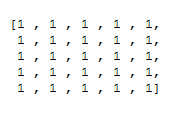
\includegraphics{images/Morphological Operations/Images/Rectangle.PNG}
  \caption{Rectangle}
  \end{figure}
\pagebreak
\item
  Diamond

  \begin{figure}[htbp]
  \centering
  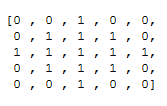
\includegraphics{images/Morphological Operations/Images/Diamond.PNG}
  \caption{Diamond}
  \end{figure}
\item
  Ellipse

  \begin{figure}[htbp]
  	\centering
  	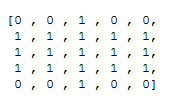
\includegraphics{images/Morphological Operations/Images/Ellipse.PNG}
  	\caption{Ellipse}
  \end{figure}
\item
  Cross

  \begin{figure}[htbp]
  \centering
  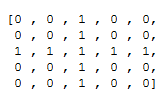
\includegraphics{images/Morphological Operations/Images/Cross.PNG}
  \caption{Cross}
  \end{figure}
\end{itemize}

\subsubsection{Morphological operations}\label{morphological-operations}

As discussed above, morphological operations are a set of techniques
used for image processing. Following are two basic morphological
operations:

\paragraph{Erosion}\label{erosion}

Erosion is a basic morphological operation applied on binary (or
grayscale) images that erodes away the boundaries of regions of
foreground pixels(i.e.~white pixels). Thus, any holes within those areas
become larger.

Erosion can be mathematically defined as- If X denotes total set of
points on the image, S denotes the set of points on the structuring
element and Sx denotes translation of T such that its origin is at x,
then erosion of X by S is set of all points x such that Sx is a subset
of X.

\paragraph{Dilation}\label{dilation}

Dilation is a basic morphological operation applied on binary (or
grayscale) images that increases the size of the foreground
pixels(i.e.~white pixels). Thus, any holes in the image shrink whereas
the boundaries of image expand.

Dilation can be mathematically defined as- If X denoes total set of
points in an image, S denotes set of all points on the structuring
element and Sx denotes translation of S such that its origin is at x,
then dilation of X by S is a set of all point x where the intersection
of X and Sx is non-empty.

\paragraph{Opening}\label{opening}

Opening operator is derived from erosion and dilation operations. Simply
put, opening is erosion followed by dilation using the same structuring
element. This operation is useful for removing noise from an image. It
is also the dual of closing operation.

\paragraph{Closing}\label{closing}

Closing operator is also derived from erosion and dilation operations.
It can be defined as dilation of an image followed by erosion. This
operator is highly useful for closing small black points on the image.
It is the dual of opening operation.

\subsection{Applications}\label{applications}

Morphological operations are used in the following fields: - Robotics :
It allows for execution through visual feedback, motion control and
recognizing and interpreting objects. - Forensics : It helps reduce
noise in fingerprint images and consequently enhance them. - Medicine :
It can help with detection of tumors, measurement of size and shapes of
organs and much more. - Radar : It can be used in target detection and
identification systems.

\section{Code}\label{code}

Let us now have a look at the available functions for the above
morphological operations in python.

\begin{verbatim}
cv2.erode(src, kernel, iterations)

This function is used for erosion where-
      src :        Image to be eroded
      kernel :     Structuring element used
      iterations : Number of iterations to be applied

cv2.dilate(src, kernel, iterations)

This function is used for dilation where-
      src :        Image to be dilated
      kernel :     Structuring element used
      iterations : Number of iterations to be applied

cv2.morphologyEx(src, op, kernel)

This function is used for opening and closing where-
      src :    Image to be opened
      op:      Morphological operation to be performed. It's values can be one of the following-
               cv2.MORPH_OPEN-  For opening
               cv2.MORPH_CLOSE- For closing
      kernel : Structuring element to be used
      
\end{verbatim}

These functions are available in cv2 package. So cv2 must be imported in
the beginning of the code.

Now, let us see how to write the code.

\begin{itemize}
\item
  All codes involving morphological operations must first import cv2
  package to use the above functions and numpy package to create the
  structural element.

\begin{Shaded}
\begin{Highlighting}[]
\ImportTok{import} \NormalTok{cv2}
\ImportTok{import} \NormalTok{numpy}
\end{Highlighting}
\end{Shaded}
\item
  Next, the image has to be read. This is done by cv2.imread(filename,
  flag) function. Flag=0 returns a grayscale image.
\end{itemize}

\begin{Shaded}
\begin{Highlighting}[]
    \NormalTok{img }\OperatorTok{=} \NormalTok{cv2.imread(}\StringTok{"example.jpg"}\NormalTok{, }\DecValTok{0}\NormalTok{)}
\end{Highlighting}
\end{Shaded}

\begin{itemize}
\tightlist
\item
  The structuring element for the morphological operation is created
  using the following code-
\end{itemize}

\begin{Shaded}
\begin{Highlighting}[]
    \NormalTok{kernel }\OperatorTok{=} \NormalTok{np.ones((}\DecValTok{5}\NormalTok{,}\DecValTok{5}\NormalTok{), np.uint8)}
\end{Highlighting}
\end{Shaded}

\begin{itemize}
\tightlist
\item
  Now we will perform morphological operations on the grayscale image-
\end{itemize}

\textbf{Erosion}

We use cv2.erode() function for this.

\begin{Shaded}
\begin{Highlighting}[]
    \NormalTok{erosion }\OperatorTok{=} \NormalTok{cv2.erode(img, kernel, iterations }\OperatorTok{=} \DecValTok{1}\NormalTok{)}
\end{Highlighting}
\end{Shaded}

\textbf{Dilation}

We use cv2.dilate() function for this.

\begin{Shaded}
\begin{Highlighting}[]
    \NormalTok{dilation }\OperatorTok{=} \NormalTok{cv2.dilate(img, kernel, iterations }\OperatorTok{=} \DecValTok{1}\NormalTok{)}
\end{Highlighting}
\end{Shaded}

\textbf{Opening}

We use cv2.morphologyEx() fuction.

\begin{Shaded}
\begin{Highlighting}[]
    \NormalTok{opening }\OperatorTok{=} \NormalTok{cv2.morphologyEx(img, cv2.MORPH_OPEN, kernel)}
\end{Highlighting}
\end{Shaded}

\textbf{Closing}

We use cv2.morphologyEx() fuction.

\begin{Shaded}
\begin{Highlighting}[]
    \NormalTok{closing }\OperatorTok{=} \NormalTok{cv2.morphologyEx(img, cv2.MORPH_CLOSE, kernel)}
\end{Highlighting}
\end{Shaded}

\begin{itemize}
\tightlist
\item
  We can display the modified image to see and compare the changes. We
  use the cv2.imshow(windowName, img) function for the same. For
  example, if you want to see the eroded image, this is the code-
\end{itemize}

\begin{Shaded}
\begin{Highlighting}[]
    \NormalTok{cv2.imshow(}\StringTok{"Eroded image"}\NormalTok{, erosion)}
\end{Highlighting}
\end{Shaded}

\begin{itemize}
\tightlist
\item
  Alternatively, we can also save the modified image with
  cv2.imwrite(name, img) function.
\end{itemize}

\begin{Shaded}
\begin{Highlighting}[]
    \NormalTok{cv2.imwrite(}\StringTok{"Eroded image.jpg"}\NormalTok{, erosion)}
\end{Highlighting}
\end{Shaded}

\begin{itemize}
\tightlist
\item
  Whenever we use cv2.imshow(), we should also include the following
  code-
\end{itemize}

\begin{Shaded}
\begin{Highlighting}[]
    \NormalTok{cv2.waitKey(}\DecValTok{0}\NormalTok{)}
    \NormalTok{cv2.destroyAllWindows()}
    
\end{Highlighting}
\end{Shaded}

Waitkey displays the image for specified milliseconds. 0 means the
window will be open infinitely until a keypress occurs.

The full code can be found
\href{https://github.com/eyantrainternship/eYSIP_2015_Marker_based_Robot_Localisation/tree/master/Task-2/Morphological\%20operations/src}{here}

\subsection{Example images}\label{example-images}

Consider the following image:

\begin{figure}[htbp]
\centering
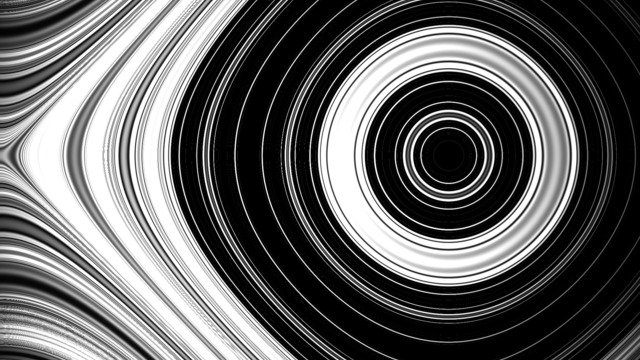
\includegraphics{images/Morphological Operations/Images/music.jpg}
\caption{Sample Image 1}
\end{figure}

On performing erosion, it looks like this:\\
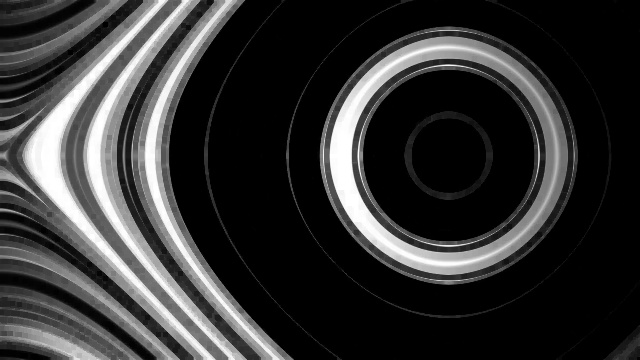
\includegraphics{images/Morphological Operations/Images/Eroded.jpg}

Notice how the concentric white boundaries of the circe almost
disappear. The black regions (holes) get bigger.

On performing dilation, the same image would look like-\\
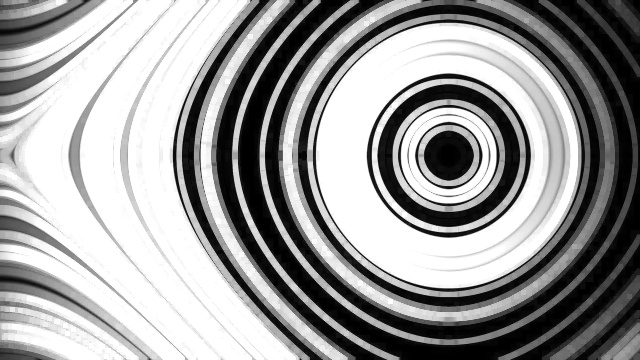
\includegraphics{images/Morphological Operations/Images/Dilated.jpg}

Here, the opposite happens. The white pixels increase whereas the black
pixels (holes) decrease.

Now, consider the next sample image:

\begin{figure}[htbp]
\centering
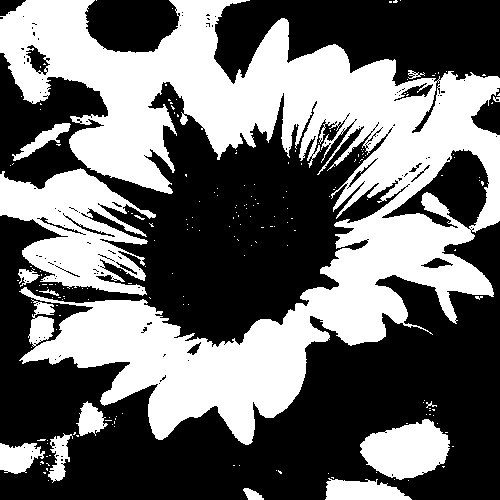
\includegraphics[width=9cm]{images/Morphological Operations/Images/Sunflower.jpg}
\caption{Sample Image 2}
\end{figure}

There are small white dots in the center of the flower whereas black
dots are littered around the petals.

When we apply opening operation on the above image, we get the following image: \\
\begin{figure}[htbp]
	\centering
	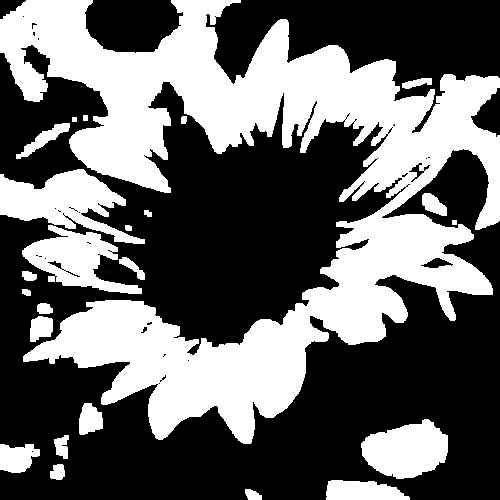
\includegraphics[width=8cm]{images/Morphological Operations/Images/Opened sunflower.jpg}
	\caption{Opened Image 2}
\end{figure}

The small white dots (noise) are removed from the image.

Now let us see the result of performing closing operation on the same:
\begin{figure}
	\centering
	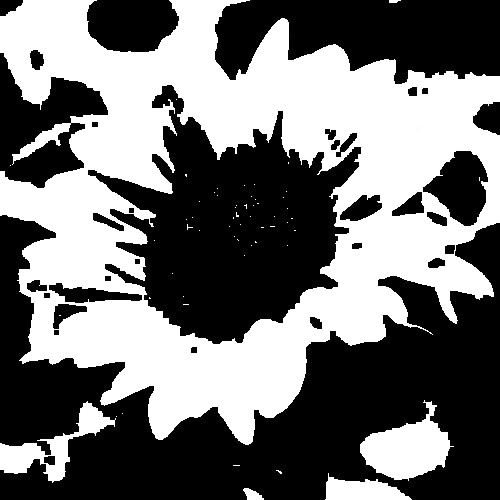
\includegraphics[width=8cm]{images/Morphological Operations/Images/Closed sunflower.jpg}
	\caption{Closed Image 2}
\end{figure}

The noise in the center of the flower is not removed but the small black
dots on the foreground(white part) are removed.
\pagebreak
\section{Resources}\label{resources}

\begin{itemize}
\tightlist
\item
  \url{http://opencv-python-tutroals.readthedocs.org/en/latest/py_tutorials/py_imgproc/py_morphological_ops/py_morphological_ops.html\#morphological-ops}
\item
  \url{http://homepages.inf.ed.ac.uk/rbf/HIPR2/morops.htm}
\item
  \url{http://www.academia.edu/3482702/Morphological_Image_Processing}
\item
  `EGGN 510 - Lecture 10-1 Morphological
  Processing'\url{https://www.youtube.com/watch?v=gmi4ah7YAi0}
\end{itemize}

\section{Exercises}\label{exercises}

\begin{itemize}
\tightlist
\item
  Perform morphological operations with different structuring
  elements(square, ellipse, diamond etc) and compare them.
\item
  Which structuring element is best suited to erode convex images while
  preserving their shapes?
\item
  Observe the effect of size of structuring element while performing
  various morphological operations.
\end{itemize}

\end{document}
